\documentclass{article}
\usepackage{a4wide}
\usepackage{amsmath, amsfonts, amssymb}
\usepackage{xcolor}
\usepackage{enumerate}
\usepackage{tikz}
\title{Algebra WS 2026}
\author{Nick Daiber}

\newtheorem{thm}{Theorem}[section]
\newtheorem{defi}[thm]{Definition}
\newtheorem{proposition}[thm]{Proposition}
\newcommand{\N}{\mathbb{N}}
\newcommand{\Z}{\mathbb{Z}}
\newcommand{\R}{\mathbb{R}}
\newcommand{\Q}{\mathbb{Q}}
\newcommand{\F}{\mathbb{F}}
\newcommand{\C}{\mathbb{C}}
\newcommand{\Mat}{\text{Mat}}
\newcommand{\ggT}{\text{ggT}}
\newcommand{\kgV}{\text{kgV}}
\begin{document}
\maketitle
\section{Ganze Zahlen und Plynome}
\begin{itemize}
    \item
           $\N_0\subset\N\subset\Z:=\{\text{zanze Zahlen}\}$
    \item
        $\Z[x]:=\{\text{Polynome mit ganzzahligen Koeffizienten}\}$\\
        $=\{a_0+a_1x+\hdots+a_nx^n|n\in\N_0,a_n\in\Z\}$
    \item
        $\Q[x]:=\{\text{Polynome mit rationalen Koeffizienten}\}$
\end{itemize}
Ein Polynom $f(x)$ definiert eine (polynomiale) Gleichung
$f(x)=0$\\
Gesucht: $\lambda$ mit $a_0+a_1\lambda+\hdots+a_n\lambda^n=0$\\
\begin{itemize}
    \item
        \color{purple}
        $2x+3=0$: Keine Lösung in $\Z$, Lösung in $\Q$
        \color{black}
    \item
        \color{purple}
        $x^2-2=0$: Keine Lösung in $\Q$, zwei Lösungen in $\R$
        \color{black}
    \item
        \color{purple}
        $x^2+2=0$: Keine Lösung in $\R$\\
        In $F_2:=\Z/_{2\Z}:=\{\overline{0},\overline{1}\}$:
        Eine Lösung
        \color{black}
    \item
        \color{purple}
        $x^2+x+1=0$: Keine Lösung in $\F_2$\\
        \color{black}
\end{itemize}
\begin{itemize}
    \item
        Gegeben $K[x],f(x)\in K[x]$: Ist $f(x)$ lösbar in $K$?
        Ist $f(x)$ irgendwo Lösbar? Wenn ja, wo?
    \item
        Gibt es immer Lösungsformeln?
\end{itemize}
\begin{thm}[Descartes]
    Sei $f(x)=x^n+a_{n-1}x^{n-1}+\hdots+a_1x+a_0$
    mit $a_i\in\Z$\\
    Sei $x_0\in\Q$ eine Lösung. Dann ist $x_0\in\Z$.\\
    \color{blue}
        Es kommt also nicht jedes $x_0\in\Q$ als Lösung vor.\\
    \color{black}
    Beweis: $a_n=1\overset{1.2}\Rightarrow (s|1)\Rightarrow
    s\in\{1,-1\}\Rightarrow x_0=\pm a_0\in\Z$
\end{thm}
\begin{thm}[Descantes]
    Sei $f(x)=a_nx^n+a_{n-1}x^{n-1}+\hdots+a_1x+a_0\in\Z[x]$\\
    und sei $x_0=\frac{r}{s}$ eine Lösung von $f(x)=0$.
    Dann ist $r\in\Z$ ein Teiler von $a_0$ und $s\in\Z$
    ist ein Teiler von $a_n$\\
    Beweis: Sei $x_0=\frac{r}{s}$, $f(x_0)=0$
    \begin{align*}
        f(x_0)&=0\\
        \Rightarrow
        a_n\left(\frac{r}{s}\right)^n+\hdots+a_0&=0&|\cdot s^n\\
        \Rightarrow
        a_nr^n+a_{n-1}r^{n-1}s+\hdots+a_1rs^{n-1}+a_0s^n&=0\\
        \Rightarrow
        r(a_nr^{n-1}+\hdots+a_1s^{n-1})&=-a_0s^n
    \end{align*}
    $r,s$ sind Teilerfremd, aber
    \begin{equation*}
        (r|-a_0s^n)\Rightarrow r|a_0
    \end{equation*}
    $s$ ausklammern:
    \begin{equation*}
        (s|-a_nr^n)\Rightarrow s|a_n
    \end{equation*}
\end{thm}
\color{blue}
$\N$ ist festgelegt durch die Peano-Axiome:
$1\in\N,\exists$ injektive (Nachfolger-) Funktion\\
$\N\rightarrow\N,n\mapsto n'(=:n+1)$ jedes $m\in\N$ ist
ein $n'$ mit Ausnahme $m=1$\\

$\underset{X\text{(Menge)}}\forall 1\in X\land
\underset{n\in\N}\forall n\in X\rightarrow n'\in X
\Rightarrow \N\subset X$

$X=\{\text{Zahlen für die Aussage $A$ Wahr}\}, A(1)=1\in X$
(Induktionsanfang)\\
$n\in X:A(n)$ wahr $\Rightarrow A(n')=A(n+1)$ wahr
(Induktionsschritt), dann ist
$\underset{m\in\N}\forall A(m)$ wahr
\color{black}
\begin{defi}
    Ein \textbf{Ring} $R$ ist ein Quintupel $(R,+,\cdot,0,1)$
    bestehend aus eine Menge $R$ mit zwei Abbildungen
    \begin{itemize}
        \item
            Addition:
               $+:R\times R\rightarrow R,(a,b)\mapsto a+b$
        \item
            Multiplikation:
               $\cdot:R\times R\rightarrow R,(a,b)
            \mapsto a\cdot b$
    \end{itemize}
    Es gilt
    \begin{itemize}
        \item
            $+$ ist Assoziativiv:
            $\underset{a,b,c\in R}\forall (a+b)+c=a+(b+c)$
        \item
            $+$ ist Kommutativ:
            $\underset{a,b\in R}\forall a+b=b+a$
        \item
            $\cdot$ ist Assoziativiv:
            $\underset{a,b,c\in R}\forall
            (a\cdot b)\cdot c=a\cdot (b\cdot c)$
    \end{itemize}
    Weiter ist $0_R\neq 1_R$
    \begin{itemize}
        \item
            Neutrales Element der Addition:
            $\underset{a\in R}\forall a+0_R=a$
        \item
            Neutrales Element der Multiplikation:
            $\underset{a\in R}\forall a\cdot 1_R=a=1_R\cdot a$
    \end{itemize}
    Es ist außerdem
    \begin{itemize}
        \item
            Inverses der Addition: $\underset{a\in R}\forall
            \underset{-a\in R}-a+a=0$
    \end{itemize}
    Es gilt
    \begin{itemize}
        \item
            Distributivgesetz:
            $\underset{a,b,c\in R}\forall
            (a+b)\cdot c=a\cdot c+b\cdot c$
    \end{itemize}
    \color{blue}
    $R$ ist ein \textbf{Kommutativer Ring}, wenn zusätzlich
    $\underset{a,b\in R}\forall a\cdot b=b\cdot a$
    \color{black}

    Eine Teilmenge $S\subseteq R$ ist ein
    \textbf{Teilring (Unterring)} von $R$, wenn $0_R,1_R\in S$
    und unter den Operationen $+_R$ und $\cdot_R$
    abgeschlossen ist. Dann gilt
    $(S,+_R,\cdot_R,0_R,1_R)$ selber ein Ring.
\end{defi}

\begin{itemize}
    \item
        $\Q[x,y]=\sum_{j,e}a_{j,e}x^jy^e$
        Polynom in zwei Variablen
    \item
        nicht Kommutativer Ring:
        $\Mat(n\times n,\Q),n\geq 2$
\end{itemize}

\begin{defi}
    Seien $R$ und $S$ Ringe. Eine Abbildung
    $\varphi:R\rightarrow S$ ist ein
    \textbf{Ringhomomorphismus}, wenn $\varphi(1_R)=1_S$ und
    $\underset{a,b\in R}\forall\varphi(a+b)
    =\varphi(a)+\varphi(b)$ und $\underset{a,b\in R}\forall
    \varphi(a\cdot_R b)=\varphi(a)\cdot_S\varphi(b)$
\end{defi}
\color{blue}
\begin{align*}
\varphi(0_R)
&=\varphi(0_R+\varphi(0_R)\\
&=\varphi(0_R)+\varphi(0_R)&-\varphi(0_R)\\
0_S&=0_S+\varphi(0_R)\\
\Rightarrow\varphi(0_R)&=0_S
\end{align*}
\color{purple}
\begin{itemize}
    \item
        Sei $R$ ein Ring, $T\subseteq R$ ein Teilring
        $\Rightarrow$ Inklusion $T\in R$ ist Ringhomomorphismus
        (nach Def. Teilring)
    \item
        $\Q\subseteq\Q[x]$
    \item
        $\Z\rightarrow \Z/_{n\Z}(n\in\N,n>1)$
\end{itemize}
\color{black}
\begin{defi}
    Sei $R$ ein kommutativer Ring.
    Ein Element $a\in R$ ist ein \textbf{Nullteiler},
    wenn $\underset{b\in R\setminus\{0_R\}}\exists
    a\cdot_R b=0_R$. $R$ ist ein Itegritätsbereich,
    wenn $0_R$ der einzige Nullteiler ist
    ($R$ ist Nullteilerfrei).
\end{defi}
In Integritätsbereichen gilt die Kürzungsregel:
$r\neq 0,r\cdot s=r\cdot t\neq 0\Rightarrow s=t$
Beweis:
\begin{equation*}
    r\cdot s=r\cdot t=0\Rightarrow \underbrace{r}_{\neq 0}
    (s-t)=0\Rightarrow s-t=0
\end{equation*}

Ein Körper ist ein Kommutativer Ring, für den gilt:
\begin{equation*}
    \underset{a\in K\setminus\{0\}}
    \forall\underset{a^{-1}\in K}\exists
    a\cdot a^{-1}=1_K
\end{equation*}
Es gilt $a=1\cdot a=(bb^{-1})\cdot a=b(b^{-1}\cdot a)$
d.h. $b$ ist ein Teiler von $a$.

$\Z,\Q[x],\hdots$ sind keine Körper

Wenn Division nicht immer funktioniert versucht man
Division mit Rest.
\begin{defi}
    Ein Integritätsbereich $R$ heißt
    \textbf{euklischer Ring} $\Leftrightarrow\exists
    \lambda:R\setminus\{0\}\rightarrow\N_0$, sodass
    $\underset{a,b\in R,b\neq 0}\forall
    \underset{q,r\in R}\exists a=qb+r$, mit
    $r=0$ oder $\lambda(r)<\lambda(b).\lambda$ heißt
    \textbf{Gradfunktion}.
\end{defi}
\color{purple}
\begin{itemize}
    \item
        $R=K$ Körper, $a=\underbrace{\frac{a}{b}}_{ab^{-1}}
        \cdot b$ (also $q=ab^{-1},r=0,\lambda$ beliebig)
    \item
        $R=\Z$ %TODO

        \begin{itemize}
            \item
                Anschaulich:\\
                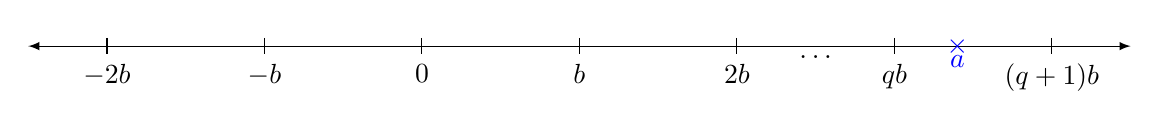
\begin{tikzpicture}
                    \draw[color=black,latex-latex] (-5,0) -- (9,0);
                    \foreach \x/\xtext in
                        {-4/$-2b$,-2/$-b$,0/$0$,2/$b$,4/$2b$,6/$qb$,8/$(q+1)b$}
                        \draw[color=black] (\x, 3pt) -- (\x, -3pt) node[below]{\xtext};
                        \draw[color=blue] (6.8,0) node[below]{$a$};
                        \draw[color=blue] node at (6.8,0) {$\times$};
                        \draw[color=black] (5,0) node[below]{$\hdots$};
                \end{tikzpicture}
                mit $a=qb+r,\underset{q\in\Z}\exists a\in[qb,(q+1)b)$
            \item
                Formal:
                $a\in\N$ gegeben, $b\in\N$,
                sei $M:=\{l\in\N|lb>a\}$
                \begin{enumerate}
                    \item
                        $M\neq\emptyset\Rightarrow
                        M\subset\N, l+q:=\min M$
                        Also $a<(q+1)b$, aber
                        $q\notin M\Rightarrow
                        qb\leq a<(q+1)b$
                    \item
                        $M=\emptyset$:
                        $a\in\N,b\in\N$, wähle $l=a:lb\geq l
                        \geq a \Rightarrow (l+1) b>a$
                \end{enumerate}
        \end{itemize}
\end{itemize}
\color{blue}
Es gilt
\begin{equation*}
    X\subseteq\N,X\neq\emptyset\Rightarrow
    \underset{n\in X}\exists\underset{m\in X}\forall
    n\leq m
\end{equation*}
\begin{itemize}
    \item ``$\Rightarrow$''
        Sei $M\subset\N$ eine Menge ohne minimales Element.
        Wir zeigen $\underset{n\in\N}\forall
        1,\hdots,n\notin M$
        \begin{itemize}
            \item Induktionsanfang:
                $1\in M\Rightarrow 1$ ist das Kleinste
                Element: Widerspruch
            \item Induktionsschritt
                $1,\hdots,n\notin M$
                Falls $n+1\in M$ ist $n+1$ das
                Minimum: Widerspruch
                $\Rightarrow n+1\notin M$
        \end{itemize}
        $\Rightarrow \underset{n\in\N}\forall n\notin M
        \Rightarrow M=\emptyset$
    \item ``$\Leftarrow$''
        Sei $X$ eine Menge mit $1\in X$ und
        $\underset{n\in X}\forall n\in X\Rightarrow n+1
        \in X$. Wir zeigen $\N\subset X$.
        Sei $M:=\N\setminus(\N\cap X)$ es ist zz.
        $M=\emptyset$.\\
        $M\subseteq \N$. Nach vorraussetzung ist
        \begin{itemize}
            \item
                $M=\emptyset$
            \item
                $M$ hat ein Kleinstes Element.
                $\underset{n\in M}\exists n$ kleinst.
                $M\subset\N\Rightarrow n\in\N,n\neq 1:
                1\in X\Rightarrow 1\in\N\cap X$, also $1\notin M$
                $\Rightarrow n>1,n=(n-1)+1=(n-1)'$, aber
                $n$ kleinst also $n-1\notin M\Rightarrow
                n-1\in\N\cap X$ Widerspruch
        \end{itemize}
\end{itemize}
\color{black}
\end{document}
